\subsection*{\textbf{Lattice used to simulate population dynamics}}
The lattice used to simulate the population dynamics of the virtual species represented the United States and Canada and individuals could only occur within the borders of the lattice (black lines in Figure \ref{fig:NA_prec}). Although each species had a specific dispersal kernel with a particular combination of maximum and mean dispersal distances (e.g., Figure \ref{fig:kernel}), individuals could only disperse to cells within the limits of the lattice. Thus, if species occurred in a cell that was close to the border of the lattice, the species dispersal kernel was modified to allow individuals to disperse only to cells within the lattice (e.g., Figure \ref{fig:kern_crop}), preventing individuals from dispersing out of the lattice. We used mean annual temperature to generate two performance curves for each species that dictated how population growth rates changed along environmental gradients. Performance curves could be symmetric or asymmetric (left-skewed), but in both curves the species would achieve maximum growth rate under the same environmental conditions though growth rates deteriorated differently away from this optimum in each curve (Figure \ref{fig:curves}). The wide range of temperature values in the United States and Canada allowed the simulation of a variety of performance curves with different characteristics (i.e., breadths and optimum) for our virtual species. 

\begin{figure}[H]
\centering
\centerline{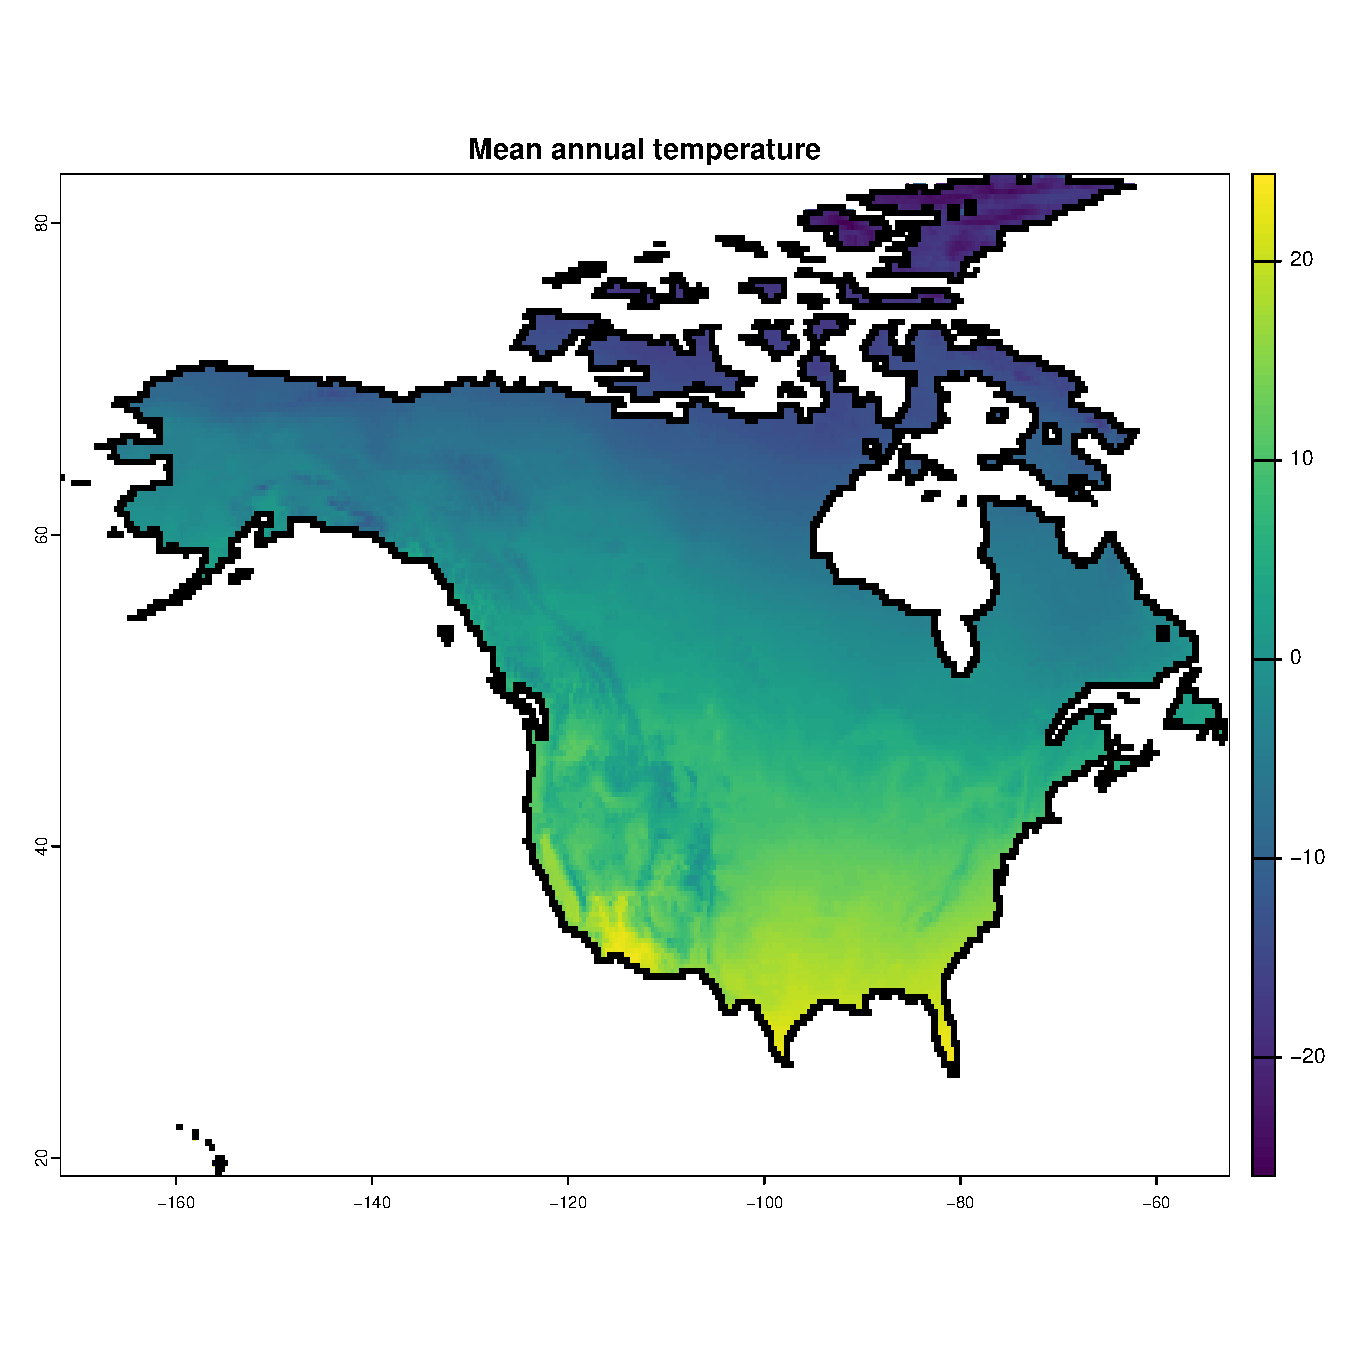
\includegraphics[width=1\textwidth]{FigsdmAbnd/NA_prec}}
\caption[Mean annual temperature in North America]{We used a lattice that had information on mean annual temperature in the United States and Canada to simulate population dynamics. Mean annual temperature values ranged from -26-24.4 $^{\circ}$C, allowing the possibility of simulating species that exist under a broad variety of environments.} 
\label{fig:NA_prec}
\end{figure}

\begin{figure}[H]
\centering
\centerline{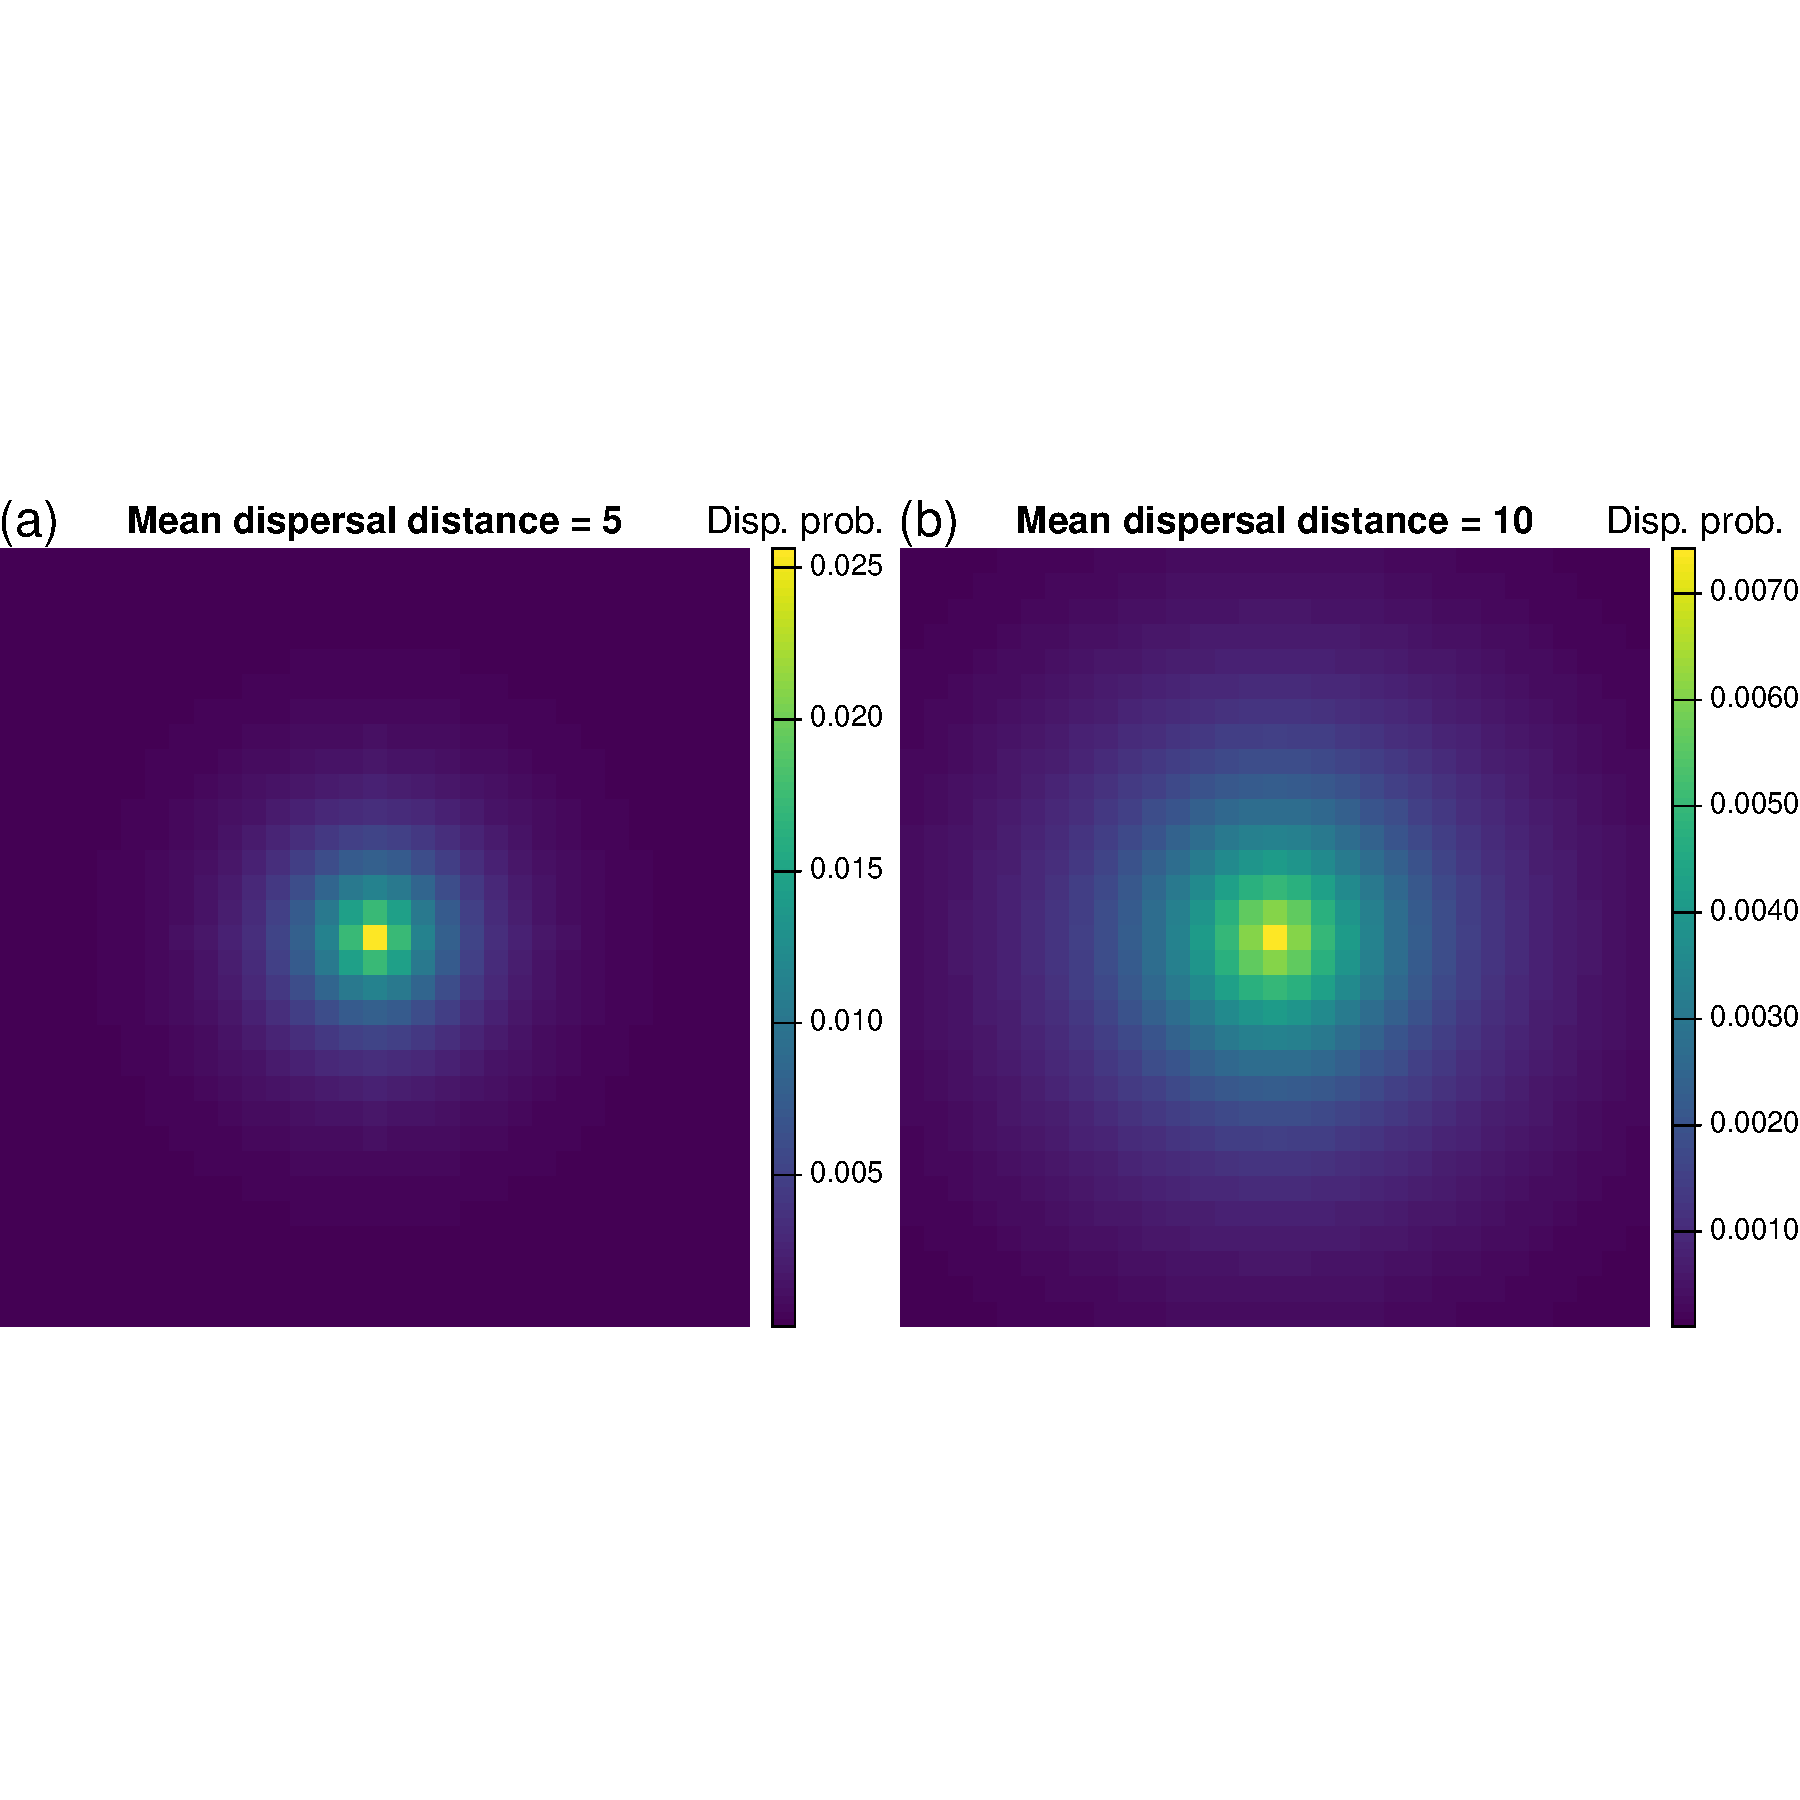
\includegraphics[width=1\textwidth]{FigsdmAbnd/kernels}}
\caption[Dispersal kernel]{A negative exponential dispersal kernel was used to simulate the dispersal of individuals between populations where each species had a dispersal kernel with specific maximum and mean dispersal distances to consider dispersal differences between species.} 
\label{fig:kernel}
\end{figure}


\begin{figure}[H]
\centering
\centerline{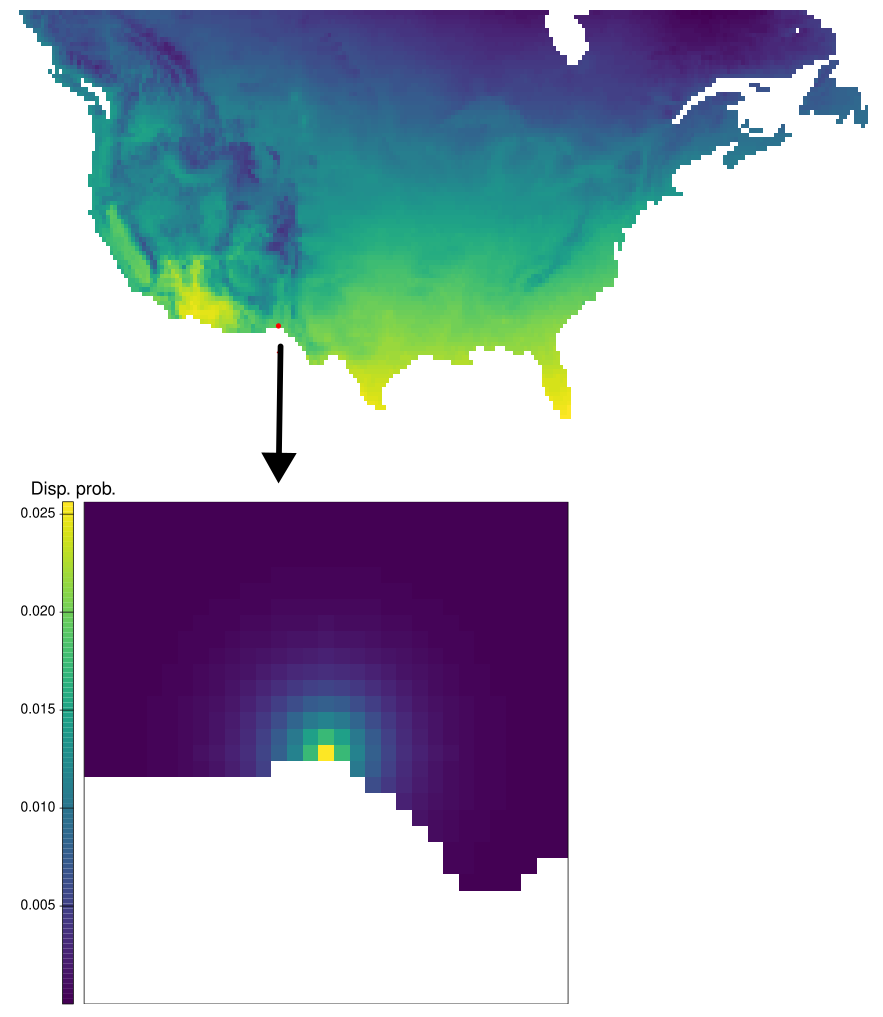
\includegraphics[width=1\textwidth]{FigsdmAbnd/kernel_crop_na.png}}
\caption[Cropped dispersal kernel]{Individuals dispersing from populations could only migrate to cells that were within the borders of the lattice representing the United States and Canada. To achieve that, only the cells of the dispersal kernel that were within United States and Canada had dispersal probabilities associated with them.} 
\label{fig:kern_crop}
\end{figure}


\begin{figure}[H]
\centering
\centerline{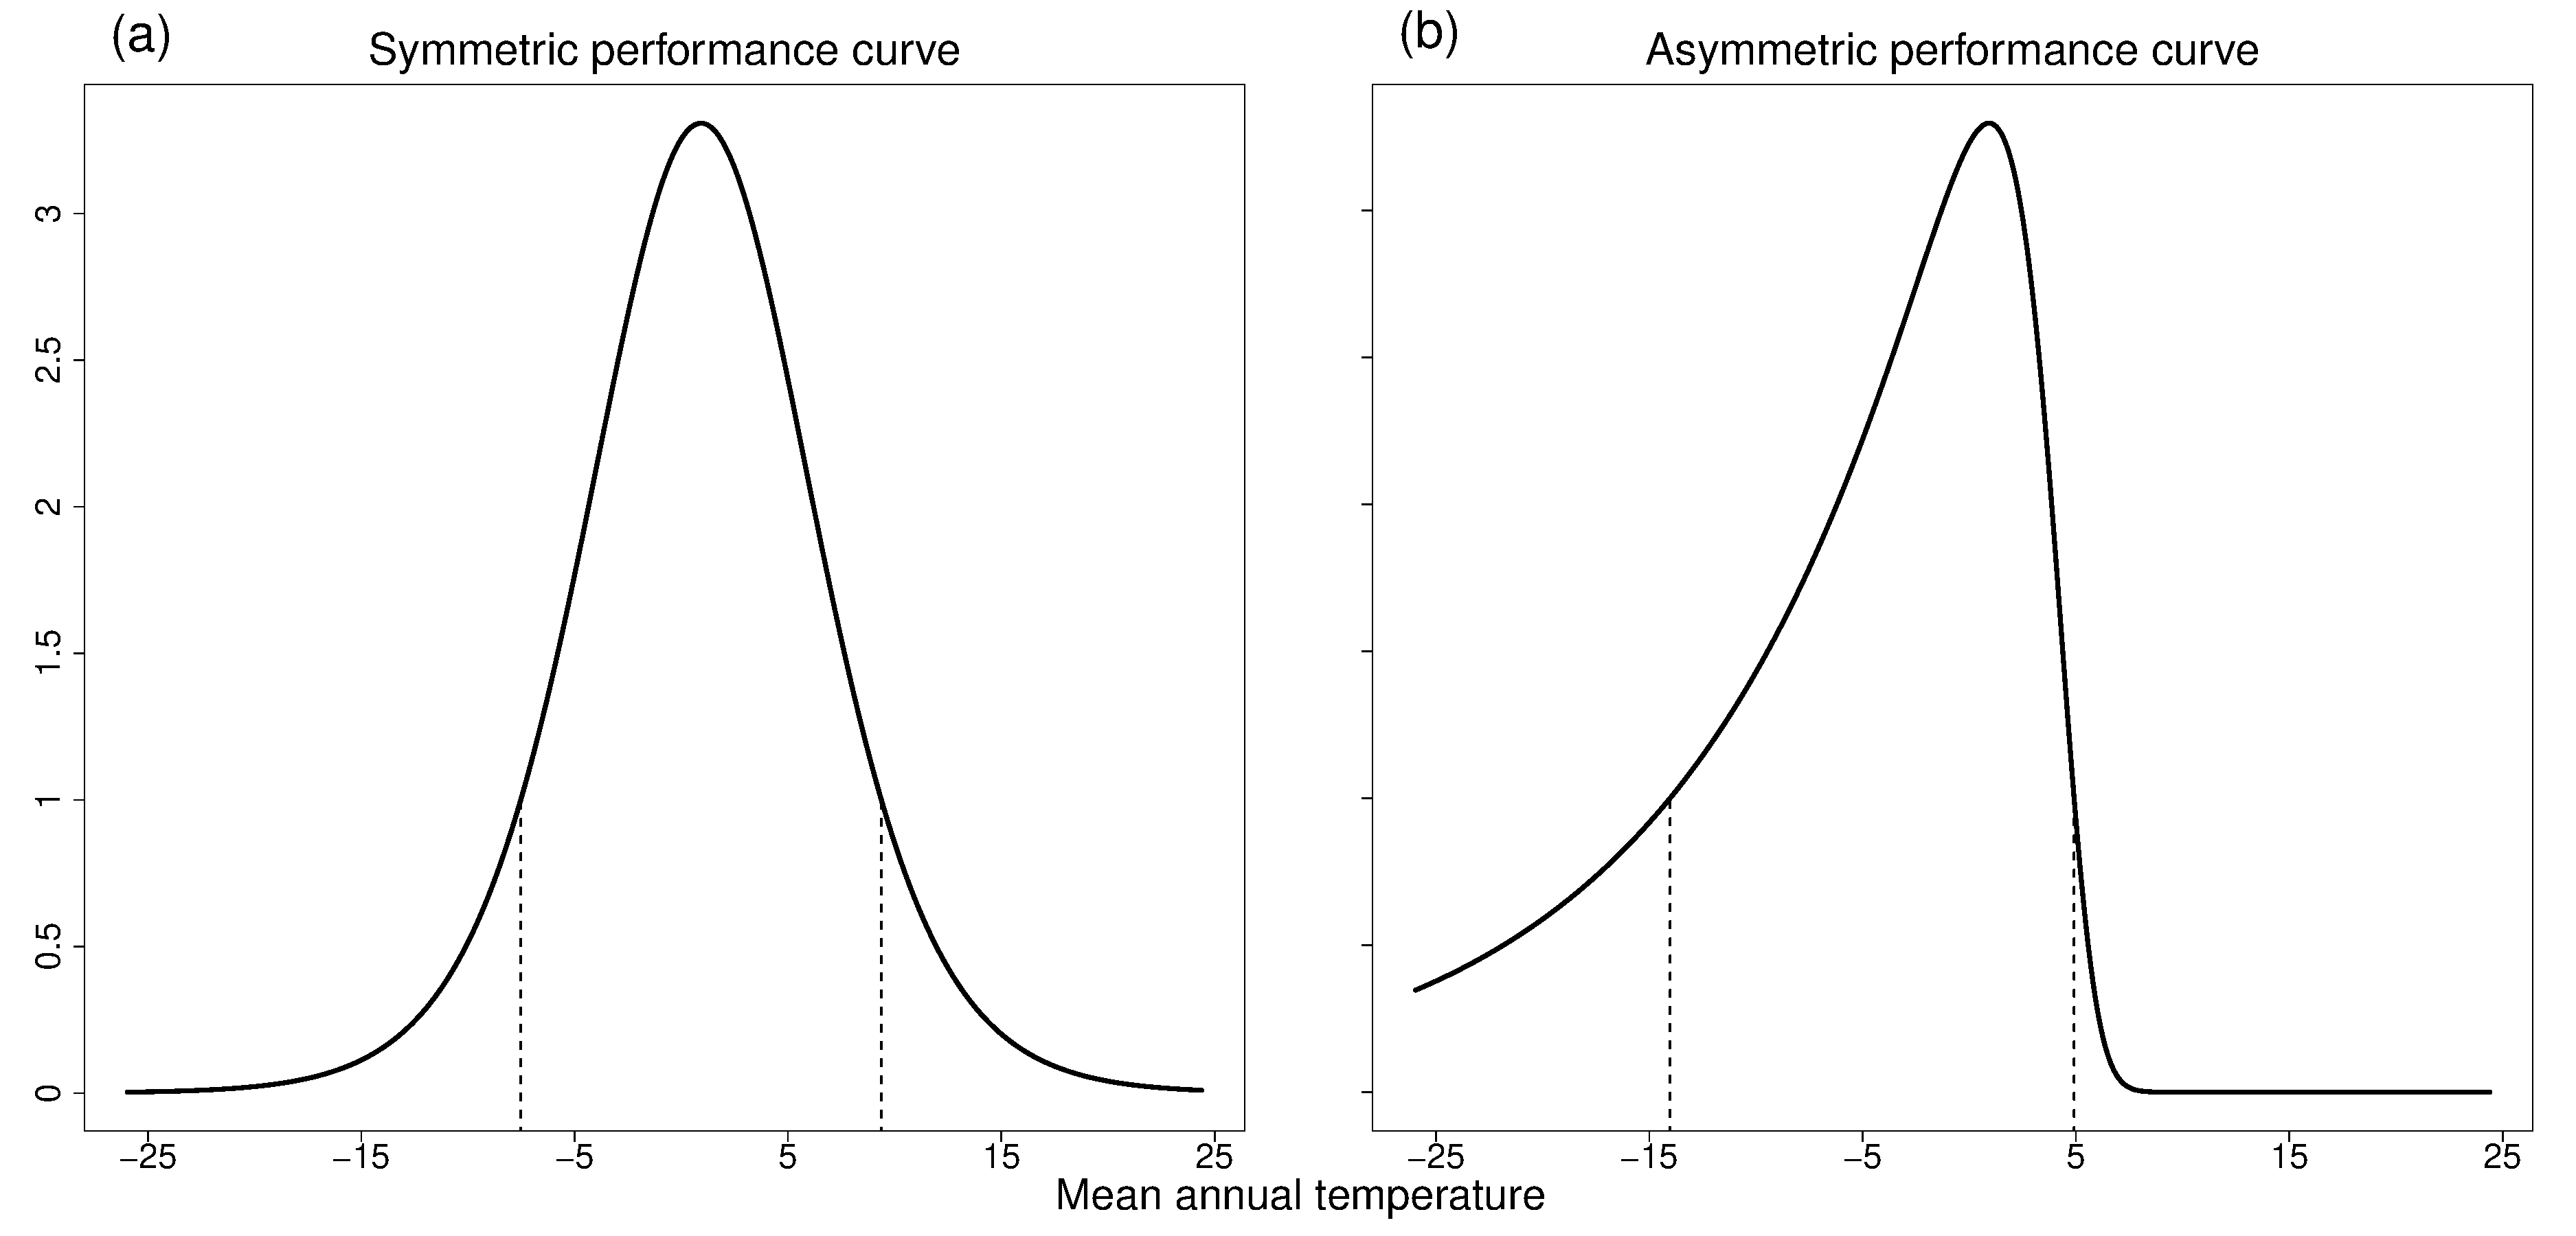
\includegraphics[width=1\textwidth]{FigsdmAbnd/performances}}
\caption[Symmetric and asymmetric performance curves]{Symmetric (a) and asymmetric (b) performance curves for a species that had an optimum mean annual temperature of 0.93 $^{\circ}$C. Dashed lines represent the range of temperatures where population growth rate is above 1 for both performance curves. } 
\label{fig:curves}
\end{figure}

\subsection*{\textbf{Linear mixed effect models diagnostic}}
Model diagnostics for the linear mixed models that we fit were done using the \texttt{performance} R package. Visual checks on the family used for our response variable, the linearity and normality of the residuals, the homogeneity of the variance, the collinearity of the predictor variables, and the normality of the random effects were performed. These visual checks indicated that these model assumptions were generally met (Figures \ref{fig:mod_dyn}-\ref{fig:mod_sp}), suggesting that our results are robust. 

\begin{figure}[H]
\centering
\centerline{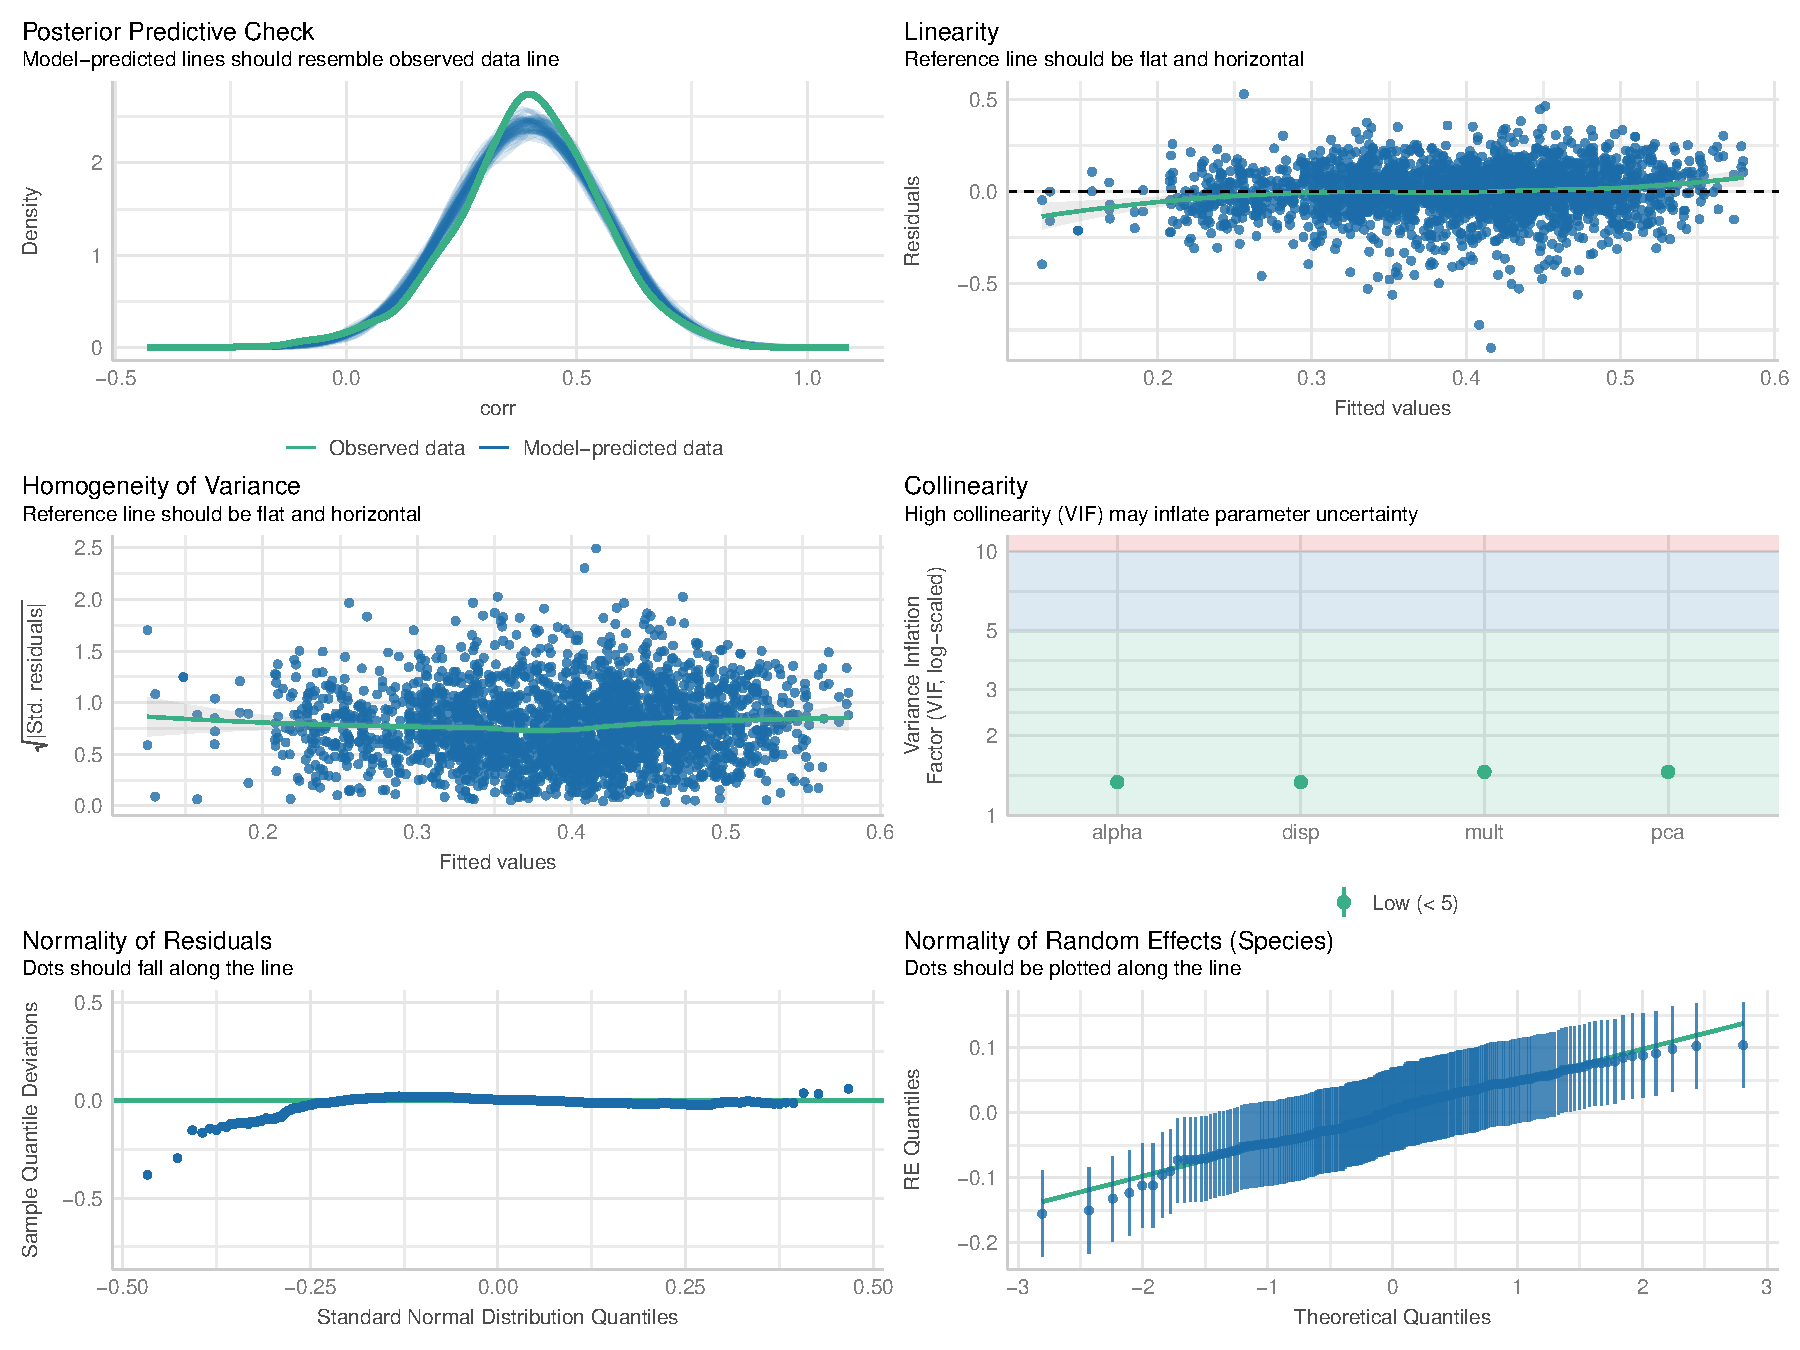
\includegraphics[width=1\textwidth]{FigsdmAbnd/mod_dyn}}
\caption[Model diagnostics for population dynamics]{Visual model diagnostics for our first linear mixed effect models presented in Figure \ref{fig:cor}. Overall, the gaussian family fits well to the response variable that we used in the models (corr), the linearity assumption is met, variance is homogeneous, there is not correlation between the predictor variables (i.e., variance inflation factor (VIF) < 5), and the residuals and the random effects are normally distributed.} 
\label{fig:mod_dyn}
\end{figure}

\begin{figure}[H]
\centering
\centerline{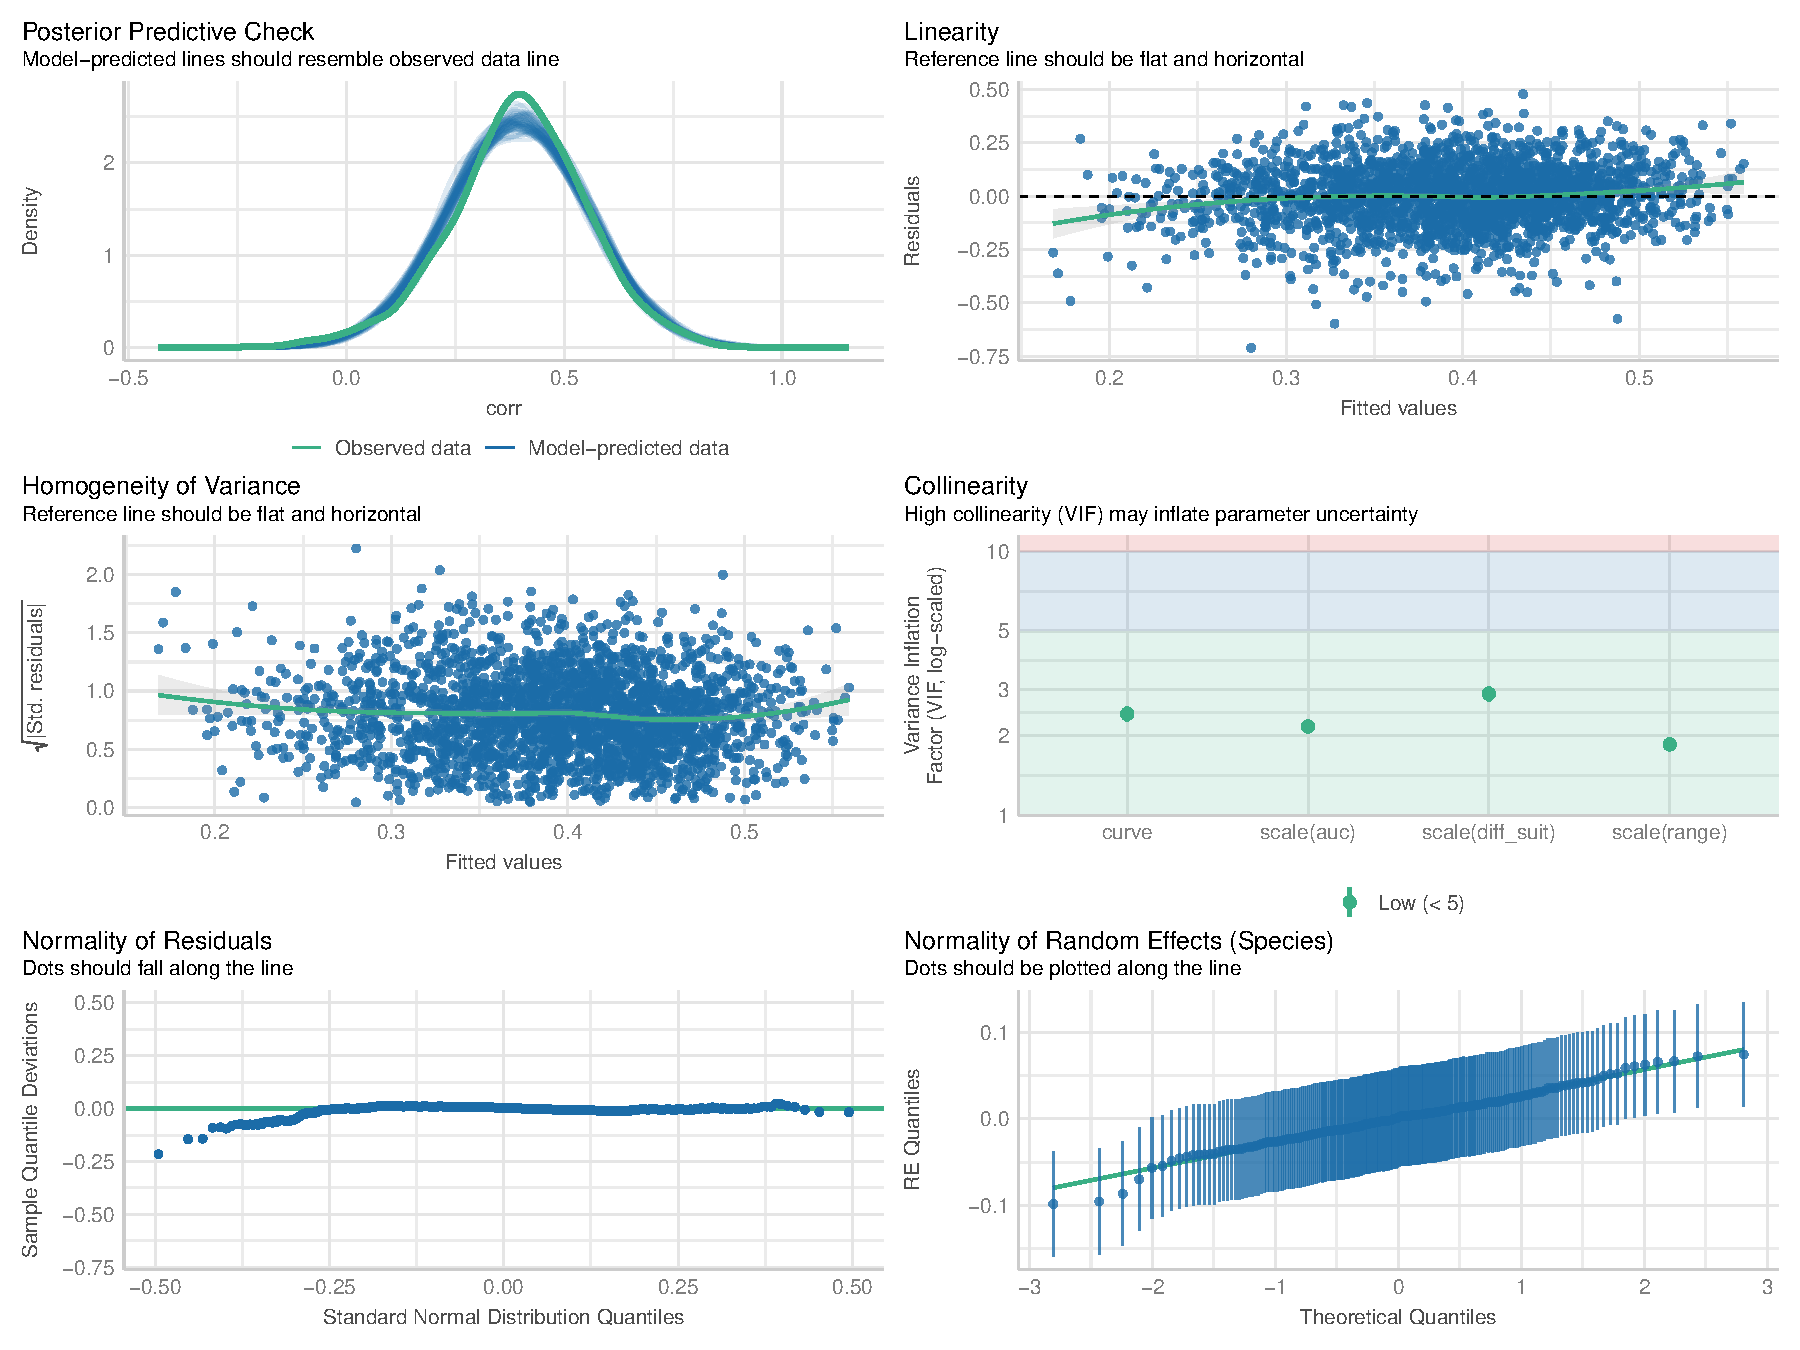
\includegraphics[width=1\textwidth]{FigsdmAbnd/mod_sp}}
\caption[Model diagnostics for species differences]{Visual model diagnostics for our second linear mixed effect models presented in Figure \ref{fig:diff}. Overall, the gaussian family fits well to the response variable that we used in the models (corr), the linearity assumption is met, variance is homogeneous, there is not correlation between the predictor variables (i.e., variance inflation factor (VIF) < 5), and the residuals and the random effects are normally distributed.} 
\label{fig:mod_sp}
\end{figure}


\subsection*{\textbf{Species distribution performance}}
The performance (AUC) of SDMs was affected by whether dispersal was considered when simulating the population dynamics of virtual species (Figure \ref{fig:auc}a). Mean performance was 0.68 and 0.72 for SDMs that were trained with occurrence data obtained from population models that considered only demographic stochasticity or demographic stochasticity and spatial variation in the strength of intraspecific competition respectively. Mean performances ranged from 0.59-0.64 for all population models that included the occurrence of dispersal events, showing a significant decrease in performance compared to when dispersal was not considered. Such decrease in SDM performance probably occurred due to the fact that, when dispersal is allowed, sink populations can be sampled and used to model the species distributions. In this case, SDM might not be able to properly detect sink populations from occurrence data, and consequently areas that are environmentally unsuitable for the species can be labeled as suitable by SDM and negatively affect performance during model evaluation. There is a negative correlation ($r$ = -0.53, $p > 0.01$; Figure \ref{fig:auc}b) between the breadth of species performance curves and SDM performance, suggesting an inability of SDMs to properly estimate the distribution of generalist species. Mean SDM performance for North American birds was 0.83. 


\begin{figure}[H]
\centering
\centerline{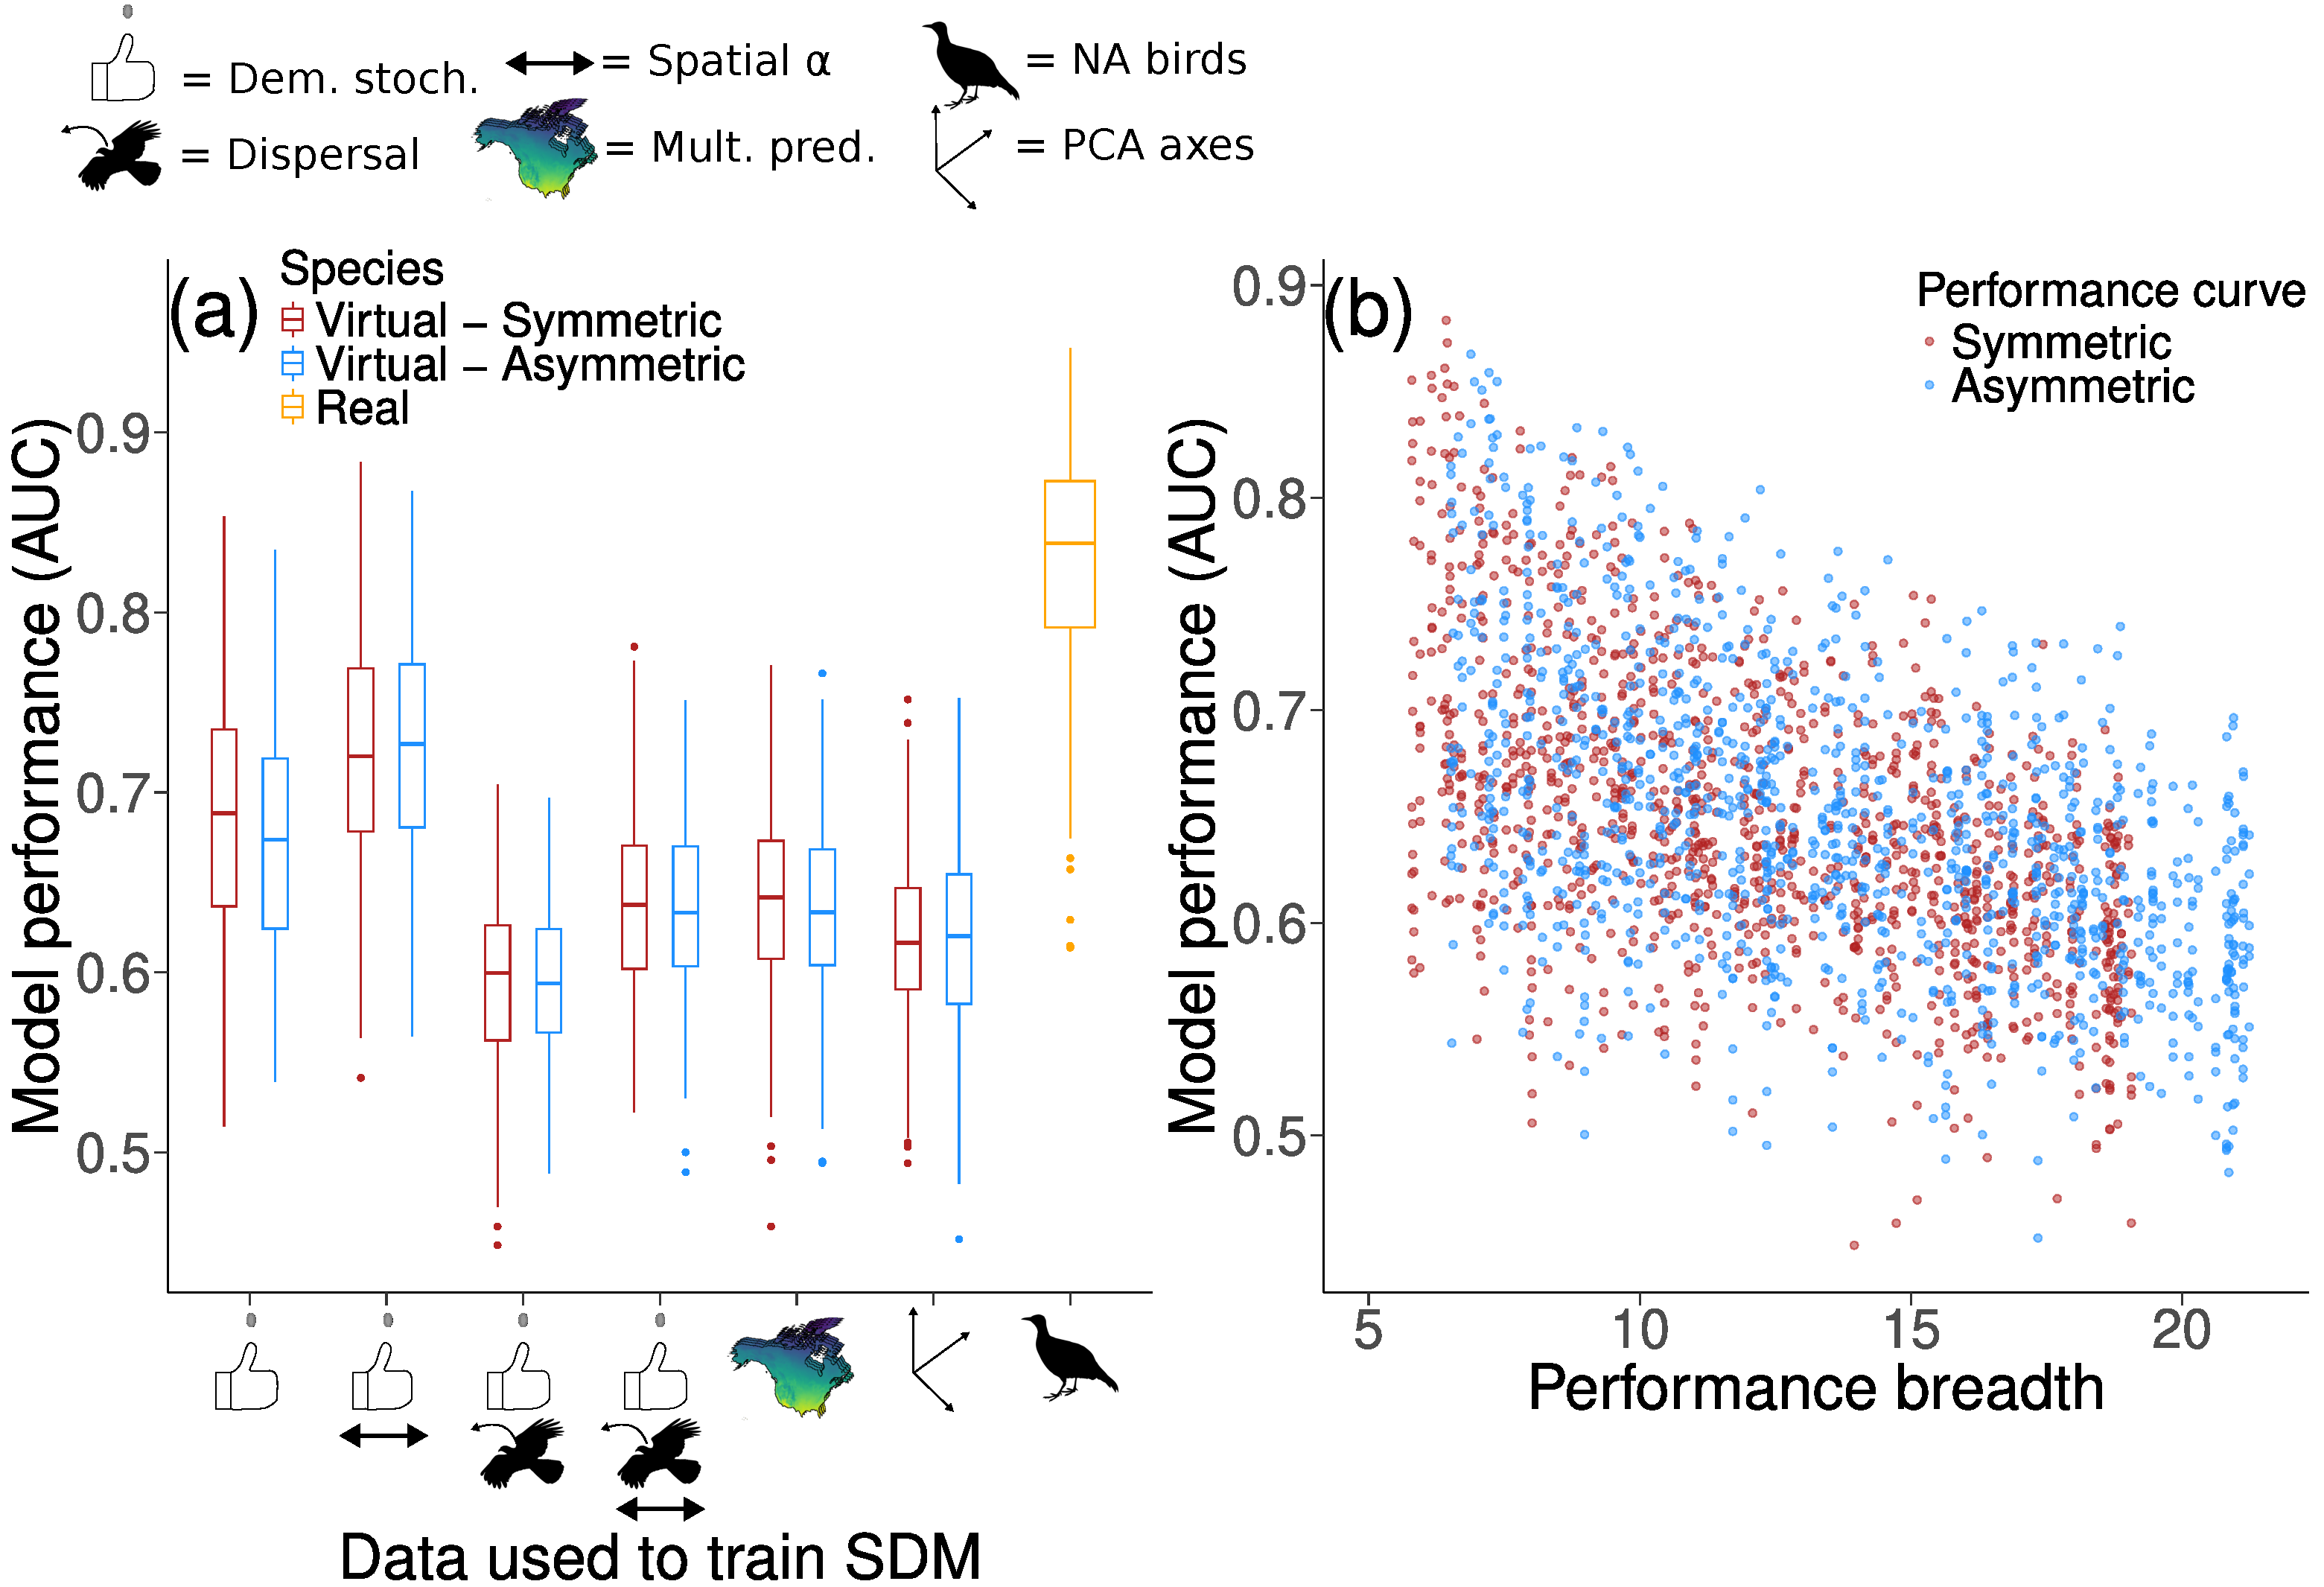
\includegraphics[width=1\textwidth]{FigsdmAbnd/Vioauc}}
\caption[Species distribution model performance]{Average model performance (AUC) observed for virtual species with symmetric and asymmetric performance curves and for North American birds.} 
\label{fig:auc}
\end{figure}

\subsection*{\textbf{Variable importance}}
SDMs that were trained with mean annual temperature and NDVI as predictors consistently identified mean annual temperature as the most important variable determining species occurrence (mean importance ranged from 79-92\%, Figure \ref{fig:imp}). When multiple environmental predictors were used to train SDM, the mean variable importance for mean annual temperature was 61\%, showing a decrease in the ability of these models in convincingly detecting the environmental condition that drives species occurrence when several environmental predictors are added to the model.


\begin{figure}[ht]
\centering
\centerline{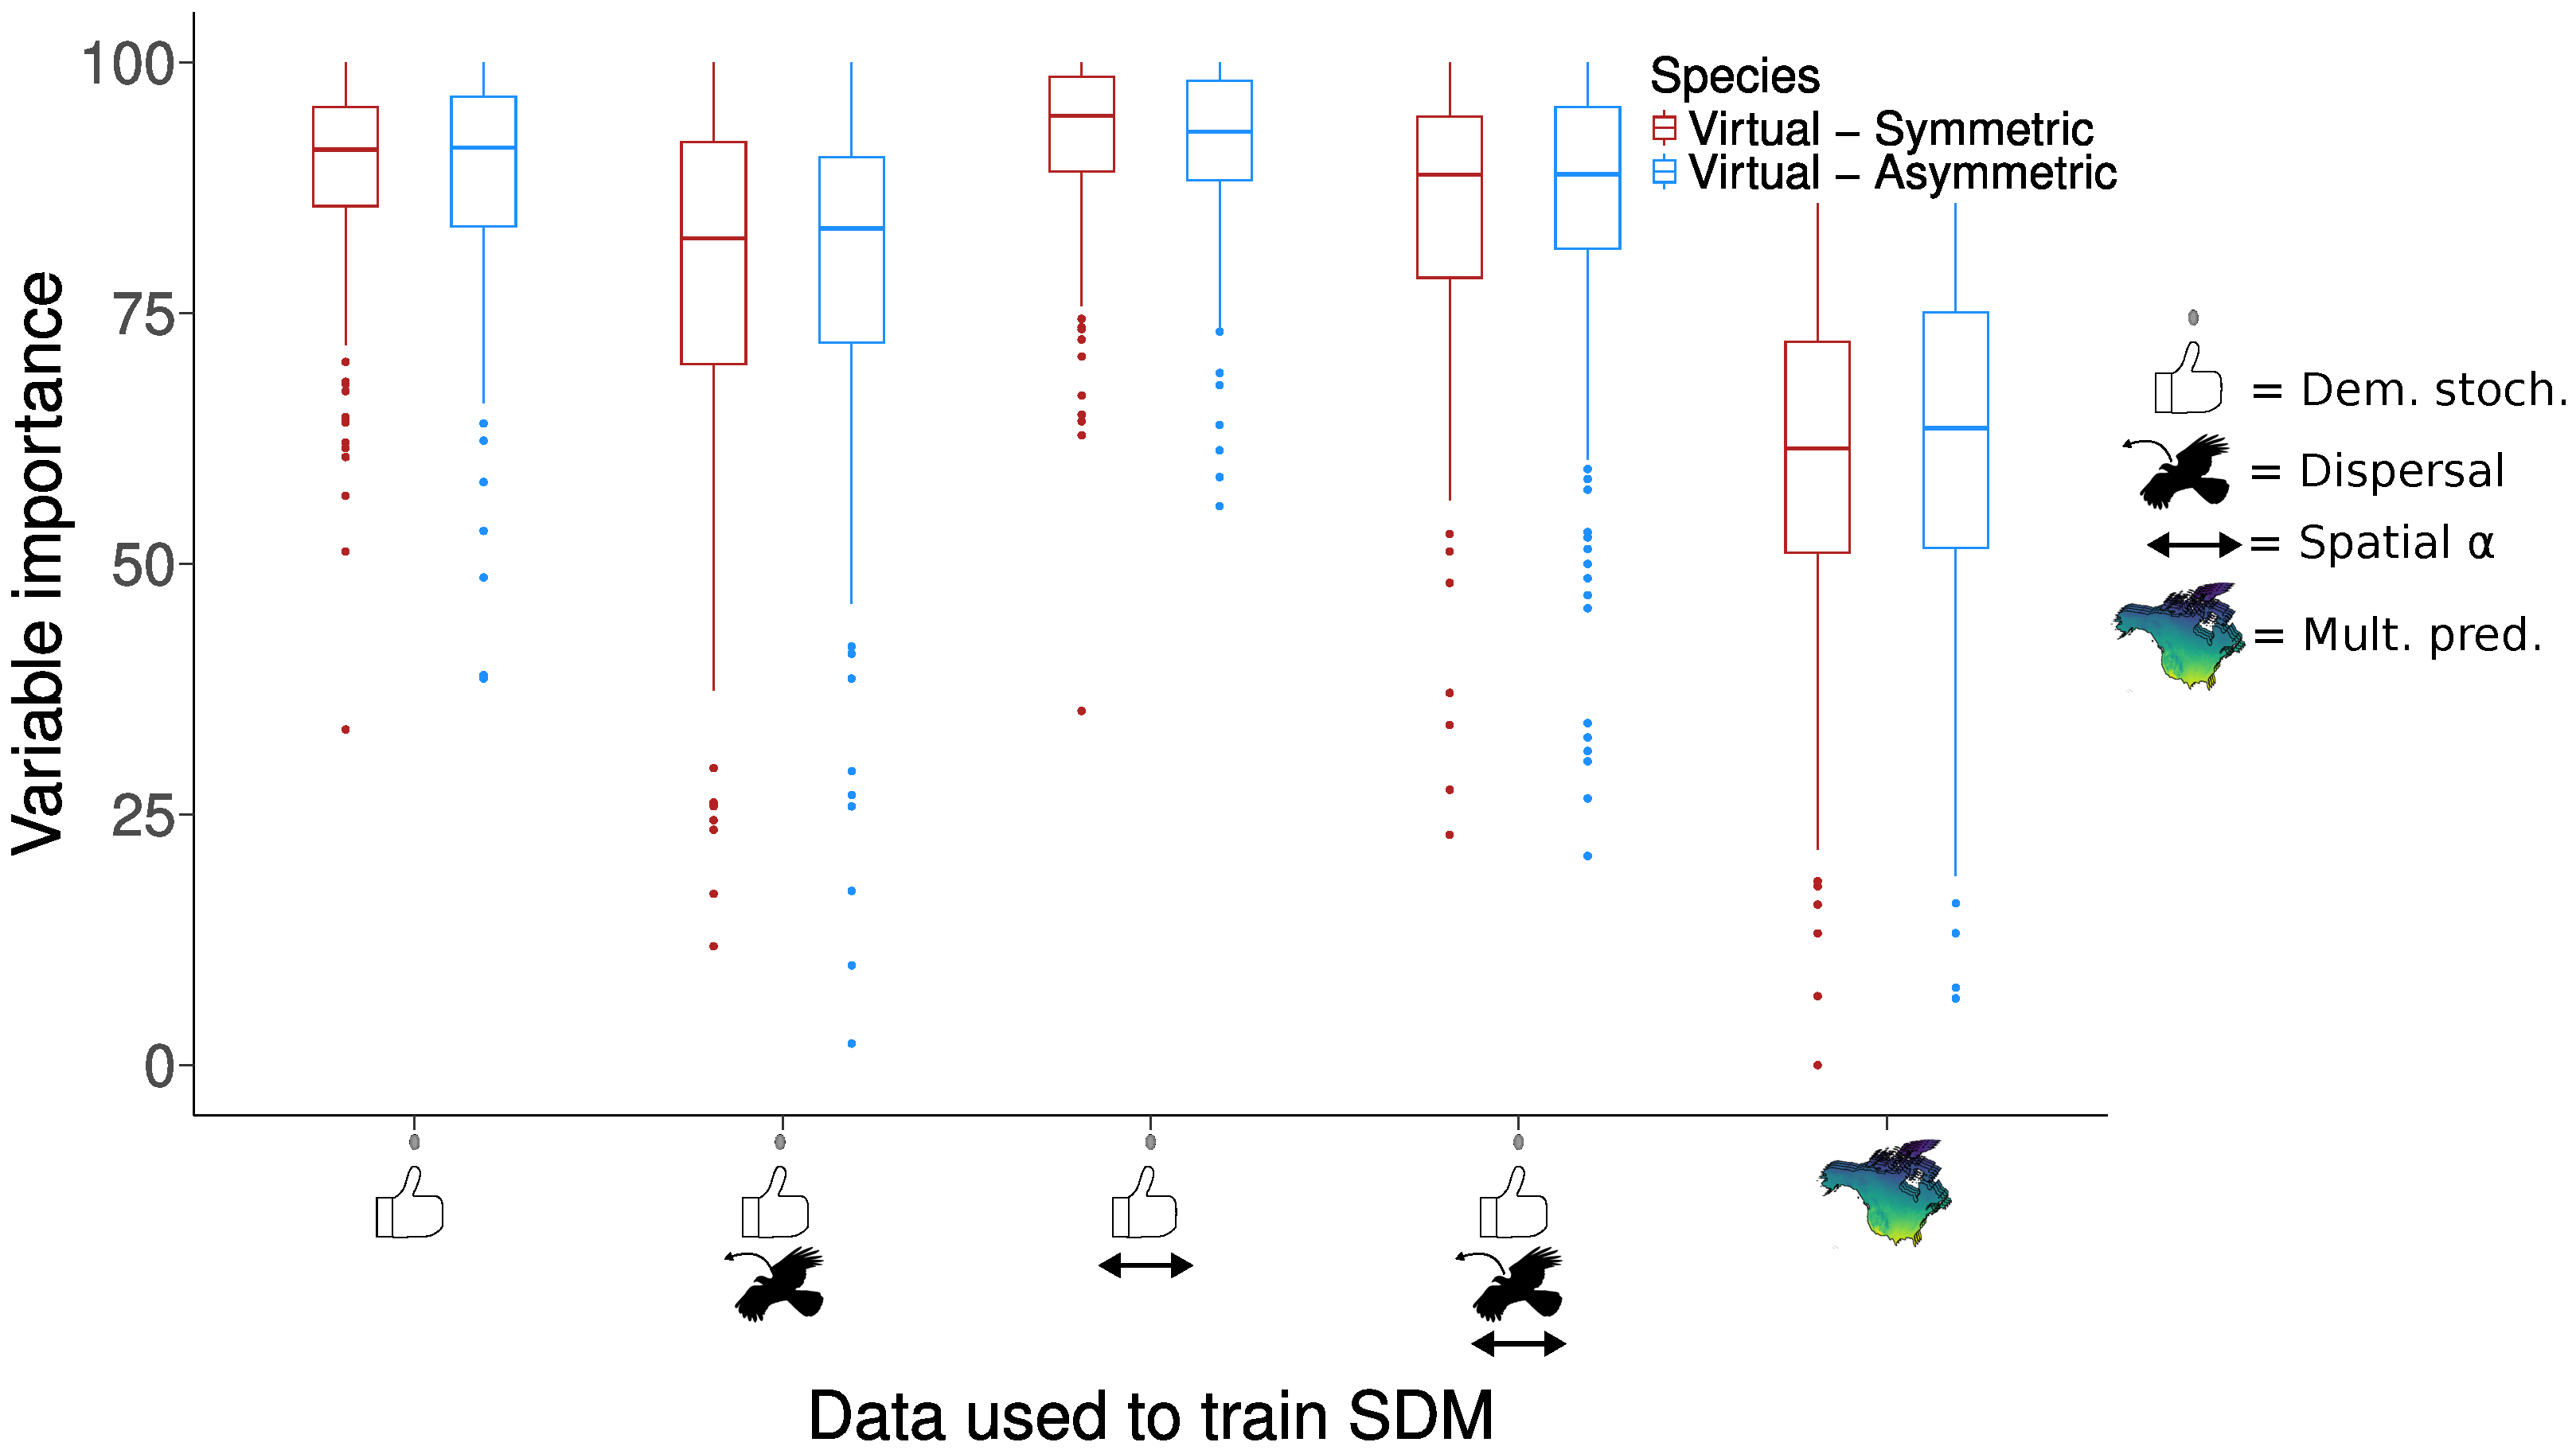
\includegraphics[width=1\textwidth]{FigsdmAbnd/impBox}}
\caption[Variable importance]{Variable importance (\%) score for mean annual temperature observed for virtual species with symmetric and asymmetric performance curves that had populations simulated considering different combinations of demographic stochasticity, spatial variation in the strength of intraspecific competition and dispersal.} 
\label{fig:imp}
\end{figure}
